\documentclass[10pt,jaurnal,compsoc]{IEEEtran}
\usepackage{caption}
\usepackage{subcaption,array}
\usepackage[pdftex]{graphicx}
\usepackage{cite}

\begin{document}
\title{Using Deep Neural Networks for autonomous UAV navigation in an apple orchard}
\author{BRESILLA, Trim}

\markboth{Inference project, Robotic Nanodegree, Udacity}%
{}
\IEEEtitleabstractindextext{%

\begin{abstract}
    With the increase of population in the world, the demand for quality food is increasing too. One of the biggest and the base of raw food production comes from Agriculture. In the recent years, due to this demand, and other enviroimental factors have heavily influenced the way agricultural production is done. Automation and robotics for fruit and vegetable production and monitoring has become the new standard. In this /paper/ we discuss an autonomous Unmanned Areal Vehicle (UAV) that would be bale to navigate through the rows in an onrchard enviroiment. The UAV is comprised of a flight controller (PIXHawk), a microcontroller (Aarduino) for analog reading from different sensors, and an On-Board Computer OBC (Raspberry Pi gen. 3). Pictres are taken through PiCamera and streamed through WiFi to a Ground Control Computer GCC running a convolutional neural network model. Based on prior trainings the model sends back to the UAV the direction to the drone using MAVLink protocol, thus performing autonomous navigation.
\end{abstract}

\begin{IEEEkeywords}
Robotics, Agriculture, Udacity, Orchard, Deep Learning.
\end{IEEEkeywords}}


\maketitle
\IEEEdisplaynontitleabstractindextext
\IEEEpeerreviewmaketitle
\section{Introduction}↓
\label{sec:introduction}

\IEEEPARstart{A}{utomation} in Agriculture is recent years i highly increasing. Eventhough Agriculture as one of the oldest occupation in the world, has seen many changes during centuries. Before Industrial Revolution was estimated that more than 80\% of population were working as farmers, while now is estimated that number to be 2\%. One of the dominant changes that characteries a growing economy is the proportionate decline in Agriculture Sector. This phenomenon is commonly atributed to two facts: food is not as demnading as other goods and services, and the rapid development of new farming technologies lead to expanding food supplies per hectare and per worker.

\begin{figure}[thpb]
      \centering
      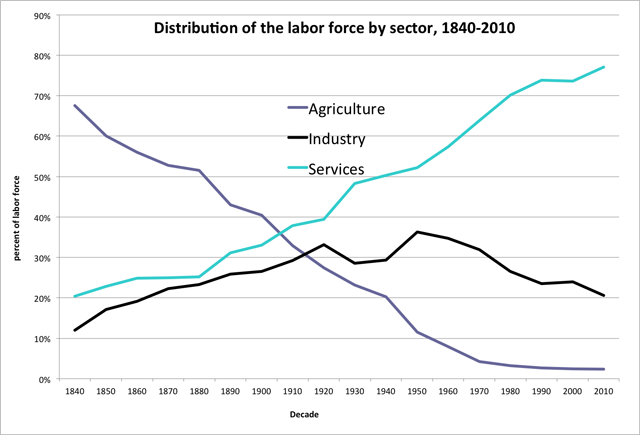
\includegraphics[width=\linewidth]{agridecline}
      \caption{Industrial Revolution.}
      \label{fig:robot1}
\end{figure}

The decrease shows significance every step of the industrial revolution. Industry 1.0 brought mechanisation, water management etc.; Industry 2.0 brought steam engines, electricity, protected enviroiments etc.; Industry 3.0 broight computers and smart apliances, GPS trctors and so on; while Industry 4.0 is foreseen to be the most significant one, bringing AI, Automation and Robotics.

The chanllenge of how we'll feed the evergrowing world populatoin in the future - is sustainable, cost-effective anf most importantly enviroimentally friendly. In order to feed 9.5 billion people that Food and Agriculture Organisation (FAO) predicts to inhabit the planet by 2050 while climate change is making more dificult to grow crops - is going to be done by Smart Farming, a high-tech and AI driven agricultural management system. Agriculture is highly repetitive, and such, many tasks can and are being automated. Individual agricultural activities on the farm takes effort, for example planting, maintaining, and harvesting crops need money, energy, labor and resources. What if we can use technology to replace some of the human activities and guarantee efficiency? That’s where artificial intelligence comes in. Agriculture is slowly becoming digital and AI in agriculture is emerging in three major categories, (i) agricultural robotics, (ii) soil and crop monitoring, and (iii) predictive analyticsi \cite{Giusti_2016}

For a farmer robot to be fully autonomus, it needs to navigate through quiet diverse and harsh enviroiment without the human supervision, then perform a set of actions at specific location like: pickin a fruit, evalute a site, spray pesticide, cut branches, plant a seed, image and scan a whole plant and take specified measurement. Controlled enviroiments like greenhouses are more managable because of controllable enviroment and better engineered, where the sensor measurements produce less nois. Whereas outdoor environment are much harsher and generaly not controllable, thus making far more difficult than indoor enviroiments. Most of outdoor robot are equiped with GPS for sensing the location, but due to accuracy, they are often companioned with other sensors like IMUs, 3DCameras, Rotary Encoders to create a sensor fusuin for a much precise action taking proces. Robots nowadays are wirelessly connected to a central operator to both receive updated instructions regarding the mission, and report status and data. However, making an autonomous farm robot requires clever controllers, localisation, communication and actioin taking systems. The technology is similar to that of autonomous cars applied to agtech. Where it differs is that farming robots often need to manipulate their environment, picking vegetables or fruits, applying pesticides in a localised manner, or planting seeds. All these tasks require sensing, manipulation, and processing of their own.

In fruit production, as is with all other fields of agriculture, crop monitoring is extremely important as there can be estimation ahead of time thus making to the farmer vere easy to pln logistics and distributions. In this paper is discussed an autonous Unmanned Areal Vehicle (UAV) flying under tree canapy, between two rows and under the anti-hail nets. In order for the robot to sucessfully follow the the row, it has firsly to know the orchard and where is the startig row, then has to percie the path between two rows while maintaining the altitude and avoind any collision with lateral branches from the trees and void any other obstacles. The approach is taken in this paper is that it considers the whole navigation as a classification task. By analysing the front face camera images, by using a convolutional neural network to classify the video / image frames stream into direction with respected weight on a single shot.

\section{Background / Formulation}
Orchards nowadays are very complex with multiple components and management procedures moving during vegetative period of the plant. There are many management decisions that often change structure and visuals of the orchard, in addition to the nature's randomity and complexity, thus making it as an ever changing organism. In this perspective, hard-coding algorithms for specific task where randomness is infinitely high is not a good approach. The path between two rows, is maintained by farmers in different ways, differently during the season, the same with the canopy, where plants starts without leaves and then later growing them. The robot itself has to fly under anti-hail nets, 1.5m above the ground, making the whole path as a corridor. Using deep learning approach the model is able to accommodate for changes and progressively learn how to navigate even when new scenarios are being dealt with.

\subsection{Materials}
The UAV/robot uses a RasbberryPi gen.3 as a On-Board Computer OBC which in turn is connected to flight controller - a PixHawk board - through serial link. The OBC due to performance limitations can not run deep-learning algorithms on its own, however its an excellent power efficient computer running full LINUX inside. It servers as intermediary layer between flight controller and other devices like more powerful computer, arduino boards with different sensors, camera, and other communication devices. The communication is done through MAVLink protocol and MAVProxy is used to multiply the device infos and status to other devices connected to it through wireless hotspot. As it runs full LINUX and Robotics Operating System ROS, with the help of MAVROS package, the whole UAV is controlled as any robot inside ROS. OBC's camera is a RaspPi Cam gen.2 which makes the image processing and encoding in its own chips, thus making it very easy to directly stream in network.

The input images taken from front-facing camera, are sent to Ground Control Computer GCC (CUDA capable) though WiFi. The computer runs the picture stream through a trained model that has three outputs: right, left, and straight. The moving average of three outputs is sent as MAVLink RC\_CHANEL\_OVERRIDE through OBC to PixHawk.


\begin{figure}[!t]
  \begin{tabular}[b]{cc}
    \begin{tabular}[b]{c}
      \begin{subfigure}[b]{0.4\columnwidth}
          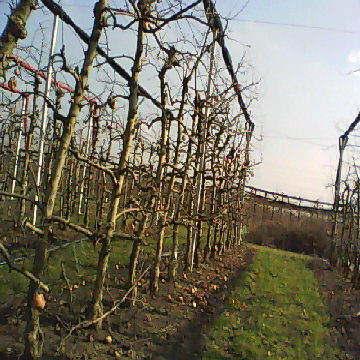
\includegraphics[width=\textwidth]{0.png} \caption{LEFT}
          \label{fig:A} \end{subfigure}\\
      \begin{subfigure}[b]{0.4\columnwidth}
          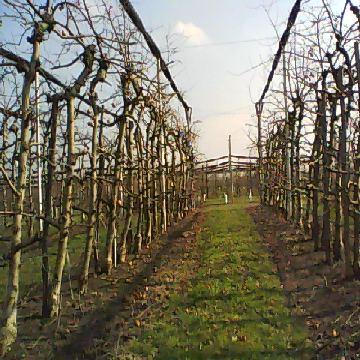
\includegraphics[width=\textwidth]{1.png} \caption{STRAIGHT}
          \label{fig:B} \end{subfigure} \end{tabular}
  & \begin{subfigure}[b]{0.4\columnwidth}
      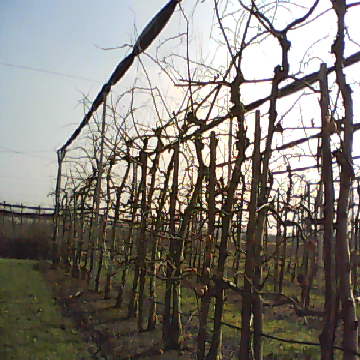
\includegraphics[width=\textwidth]{2.png} \caption{RIGHT}
      \label{fig:C} \end{subfigure} \end{tabular} \label{fig:ABC}
      \caption{Images taken from UAV - winter (trees without leaves)} \end{figure}

\begin{figure}[!t]
  \begin{tabular}[b]{cc}
    \begin{tabular}[b]{c}
      \begin{subfigure}[b]{0.4\columnwidth}
          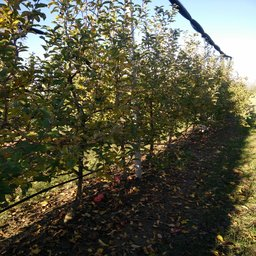
\includegraphics[width=\textwidth]{0a} \caption{LEFT}
          \label{fig:A} \end{subfigure}\\
      \begin{subfigure}[b]{0.4\columnwidth}
          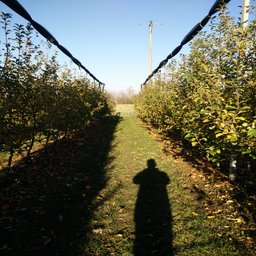
\includegraphics[width=\textwidth]{1a} \caption{STRAIGHT}
          \label{fig:B} \end{subfigure} \end{tabular}
  & \begin{subfigure}[b]{0.4\columnwidth}
      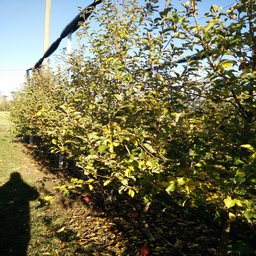
\includegraphics[width=\textwidth]{2a} \caption{RIGHT}
      \label{fig:C} \end{subfigure} \end{tabular} \label{fig:ABC}
      \caption{Images taken manually - autumn (trees with leaves)} \end{figure}

\subsection{Data Acquisition}
Data collection is done through the camera of the OBC in the UAV moving inside the orchard, controlled manually with radio controller. When OBC starts, it automatically launches few scripts (the process is managed with crontab):
\begin{enumerate}
    \item Connect to known WiFi if any exist, else create hotspot
    \item Use MAVproxy protocols to sent and receive flight plans and commands
    \item Automatically output camera stream to network
\end{enumerate}
In the GCC, the camera feed is piped from network with netcat to a python program. The program takes the camera input, divides in frames, labels it and saves in a proper dataset.

The UAV is flown very carefully inside the rows while streaming the camera feed to GCC. The flight is done many times in different rows and directions. However there have been three modes/categories, and for each mode a thousand pictures/frames were taken and labeled accordingly:
\begin{enumerate}
    \item LEFT: The drone would fly closer to the left row, and/or yawed (facing) the left side. Data collected were labeled as LEFT, model would return LEFT and RIGHT CHANNEL OVERRIDE would be sent. Fig \ref{fig:A}.
    \item STRAIGHT: The drone would fly the best position as much as it can, in the middle of the row, facing straight and having both rows symetrical to each other. Data collected were labeled as STRAIGHT, model would return STRAIGHT and FORWARD CHANNEL OVERRIDE would be sent. Fig \ref{fig:B}.
    \item RIGHT: The drone would fly closer to the right row, and/or yawed (facing) the right side. Data collected were labeled as RIGHT, model would return RIGHT and LEFT CHANNEL OVERRIDE would be sent. Fig \ref{fig:C}.
\end{enumerate}
Pictures were captured during daytime in early late winter of 2018. Daytime is important as the RasPiCam is very sensitive to light quality and light exposure.

In addition to this dataset, another set of images is used. The later set is taken manually (using smartphone camera), but during autumn of 2017, while the tree had leaves and the chlorophyll was still green. The set has 100 images per mode/category. This number discussed in results in details, proved to be very small. However the same model is run through both sets separately, and then together too.
\subsection{The Model}
To better manage different datasets and models, Nvidia's Deep Learning GPU Tranining System (DIGITS) is used. DIGITS is not in itself a machine-learning framework, rather is a wrapper for most used frameworks available. It simplifies the commonly machine-learning tasks such as managing datasets including train/validation/test splitting, designing and training different neural networks (on CUDA capable GPUs), real-time monitoring of the training process and visualisation of the process.

GoogLeNet is used as a DNN classifier. Because of the use of Inception modules, GoogLeNet is more versatile and computationaly less expensive. A simple 3x3 kernel with 256 input channels and 256 output, would have an amount of 9x256x256 calculations. Such a network where every output is connected to every input, is referred as dense connection. And while in most of CNNs activation layer for those connection is often either zero or not valuable, proving that not all those input channels are connected to output ones. Despite many techniques developed to cut off those uneccesarly connections, the computation needed is huge. Inception module of the model we chose to work with approximates a sparse CNN with a normal dense construction, and since the effective number is low (because of zeros and uneccesarly activations) the number of convolutional filters is kept small. In addition it uses convolutions of different sizes to capture details at different scales (5x5, 3x3) And it uses the so called bottleneck layer 1x1, for reduction of computation requirements.
GoogLeNet is a 27 layer deep CNN, with 22 convolution and inception layers and 5 pooling layers. However the overall number of the independent blocks is well over 100.

\begin{figure}[thpb]
    \centering
      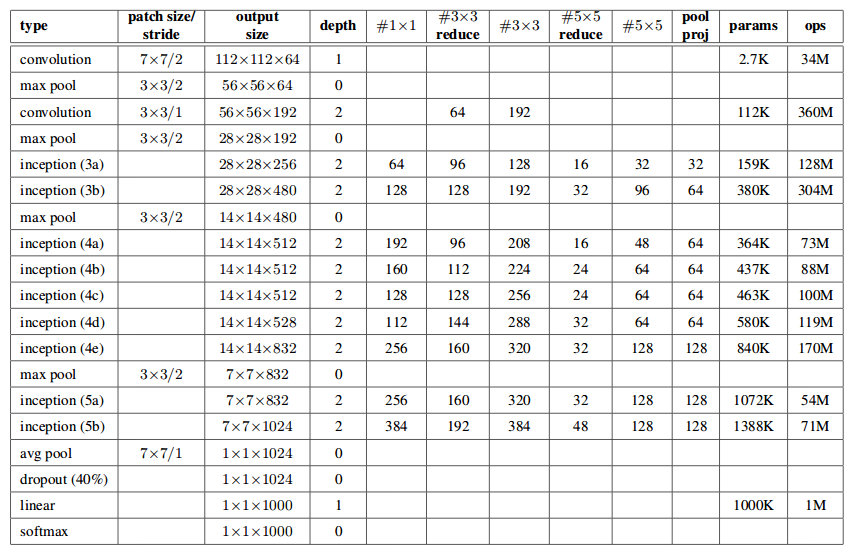
\includegraphics[width=\linewidth]{googlenet}
      \caption{GoogLeNet model structure}
      \label{fig:robot1}
\end{figure}

\subsection{Training}
Nvidia's DIGITS dealt with spliting training, validation and testing set. We decided to keep 15\% of images for training and 5\% for testing. Each images was of size 256x256. Later on we augmented (manualy with a script), all LEFT images could be mirrored and produce RIGHT image and vice versa, while STRAIGHT images when mirrored created another STRAIGHT image. The model was trained for 60 epochs in Amazon's AWS S3 instance with NVIDIA's Tesla K80 with 12GB Memory. An Adaptive Movement Solver (ADAM Optimiser) with 0.002 base learning rate was chosen. A sigmoid decay of gamma 0.08 learning rate with 60 steps is used.

\begin{figure}
      \centering
      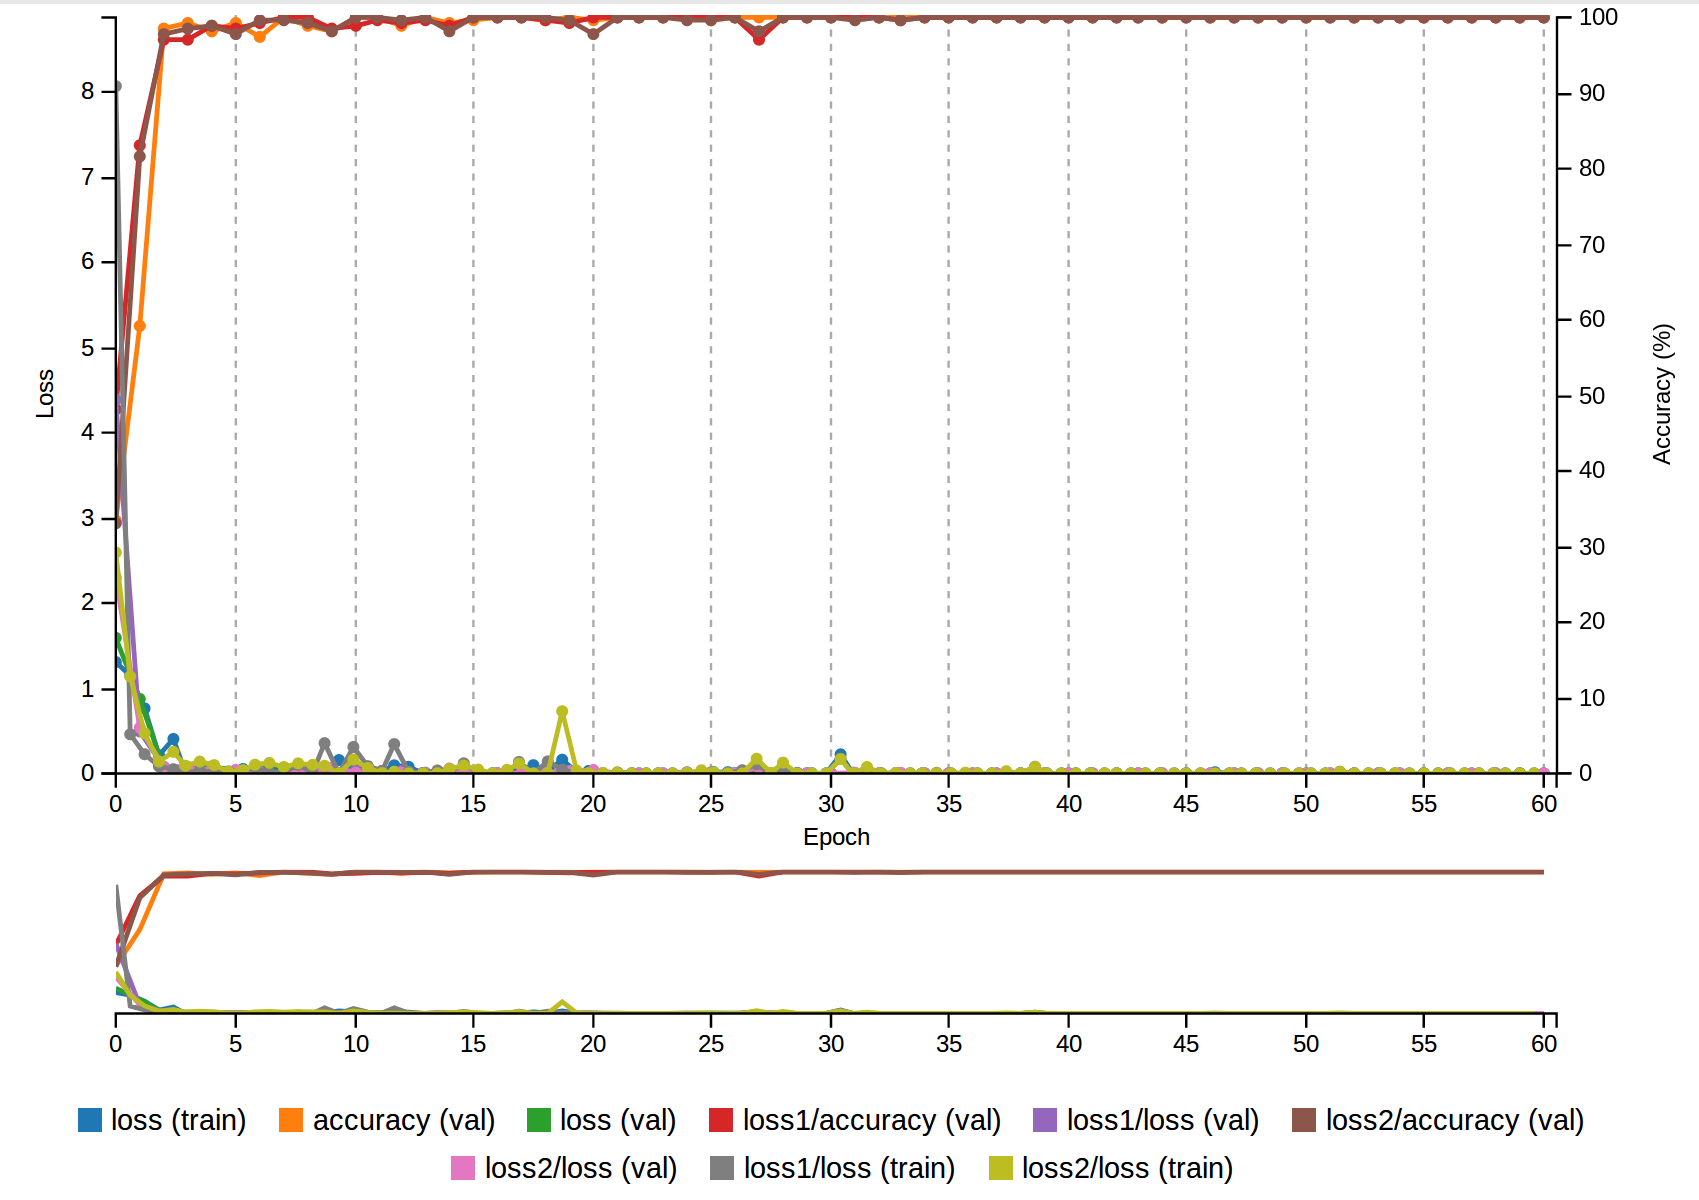
\includegraphics[width=\linewidth]{training}
      \caption{Training on 60 epochs}
      \label{fig:robot1}
\end{figure}

\begin{figure}
      \centering
      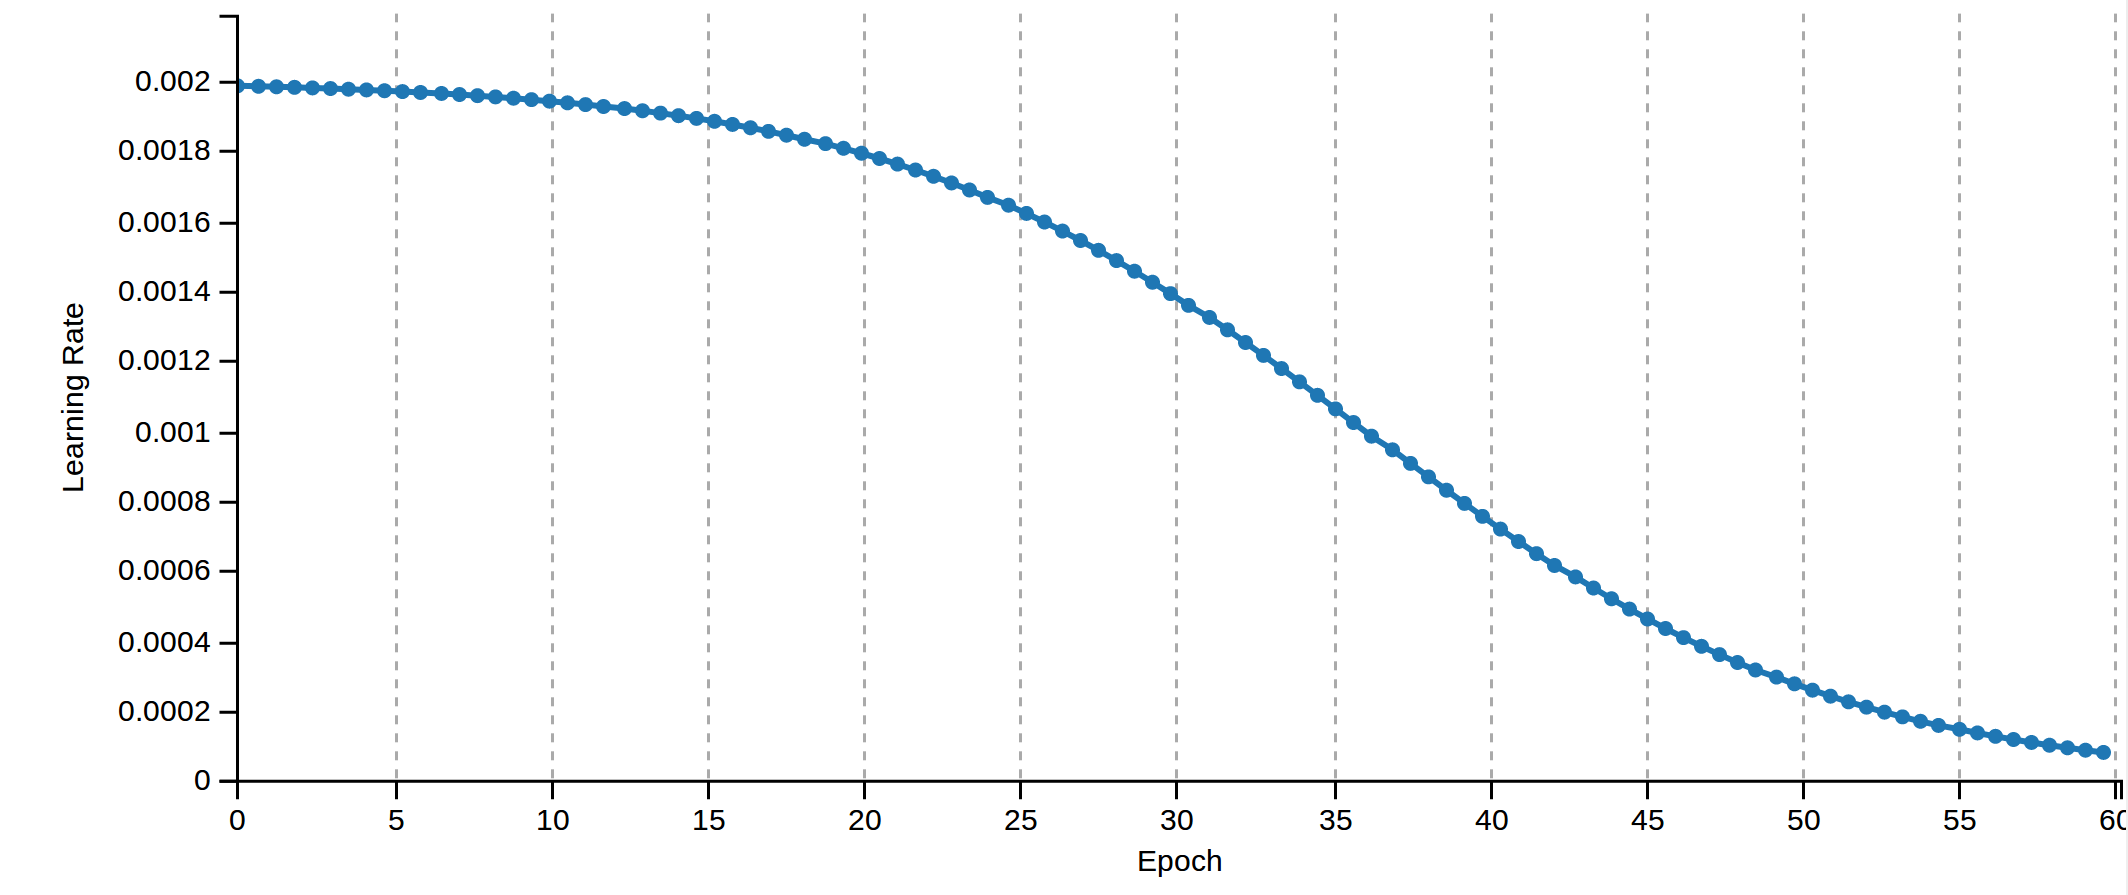
\includegraphics[width=\linewidth]{learning}
      \caption{Learning rate}
      \label{fig:robot1}
\end{figure}



\section{Results}

\begin{figure}
\centering
\subcaptionbox{LEFT}{%
  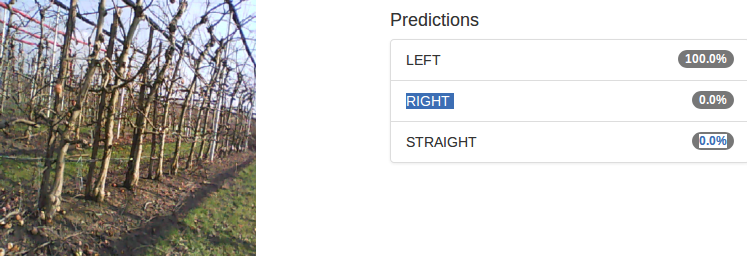
\includegraphics[width=0.45\textwidth]{left-prediction}%
  }\par\medskip
\subcaptionbox{STRAIGHT}{%
  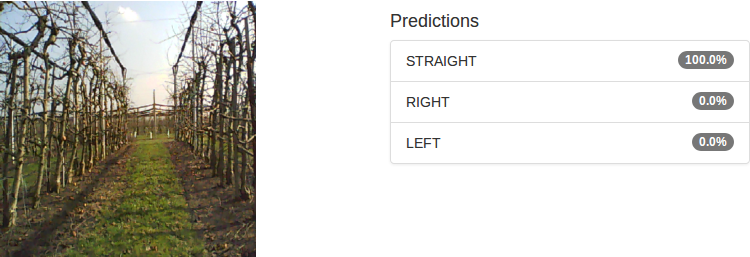
\includegraphics[width=0.45\textwidth]{straight-prediction}%
  }\par\medskip
\subcaptionbox{RIGHT}{%
  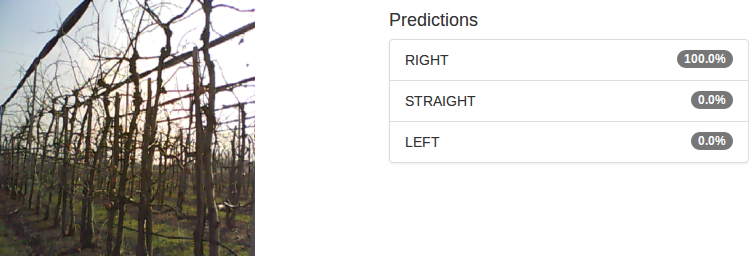
\includegraphics[width=0.45\textwidth]{right-prediction}%
  }
\caption{Predictions per class}
\label{TS}
\end{figure}

\begin{figure}
\centering
\subcaptionbox{LEFT}{%
  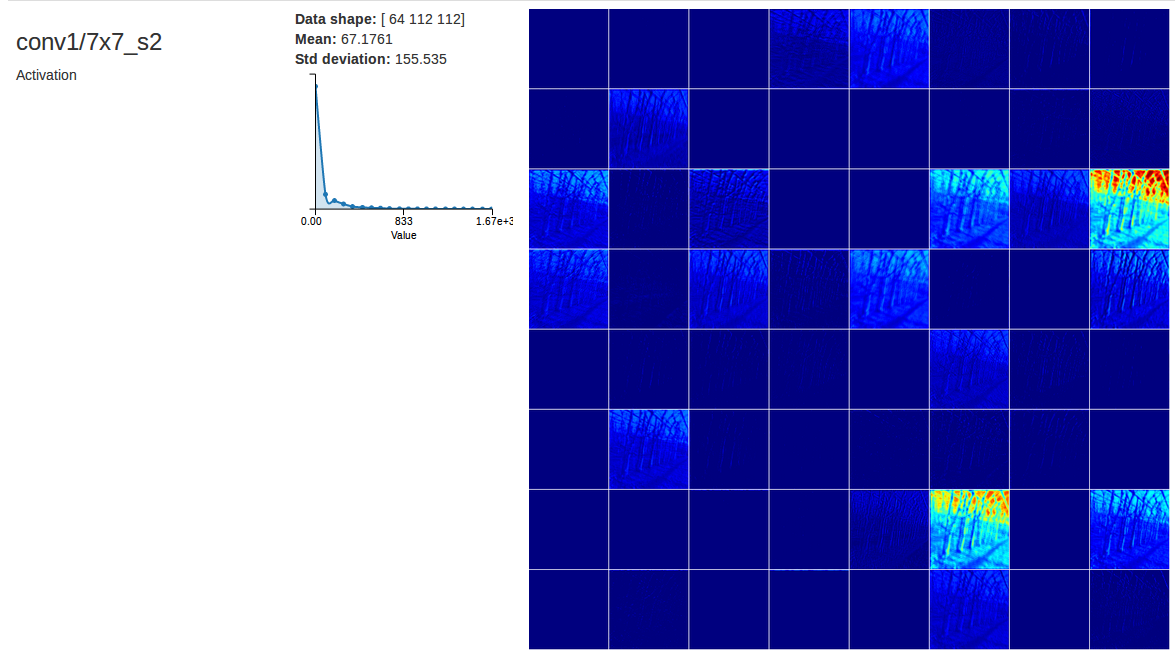
\includegraphics[width=0.45\textwidth]{left-activation}%
  }\par\medskip
\subcaptionbox{STRAIGHT}{%
  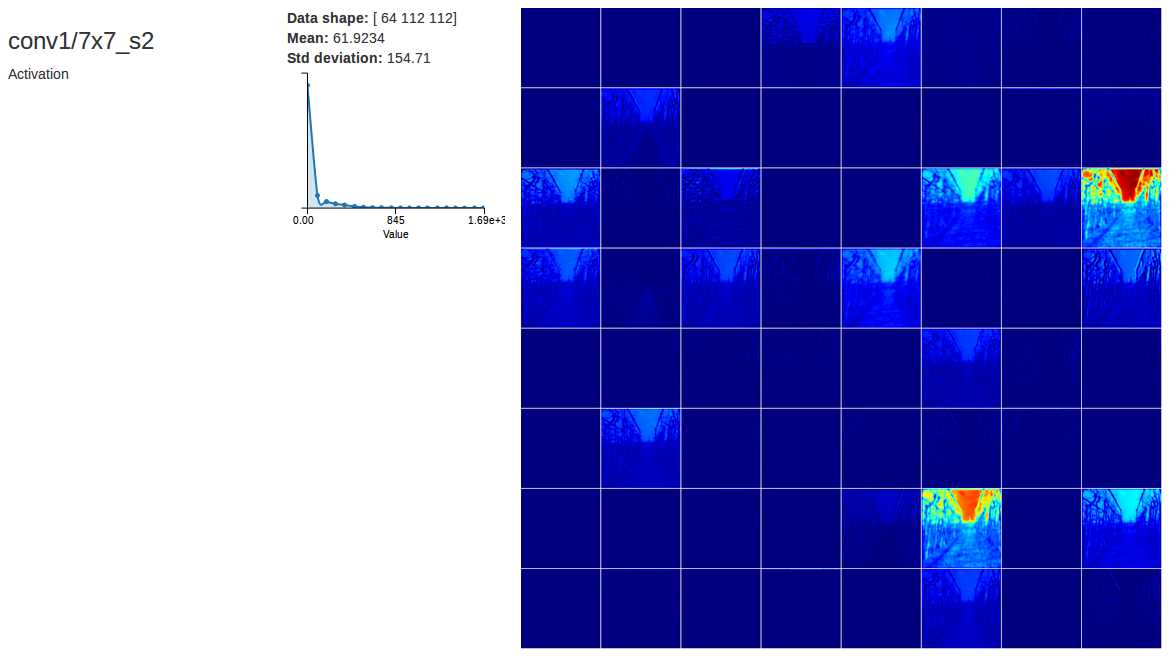
\includegraphics[width=0.45\textwidth]{straight-activation}%
  }\par\medskip
\subcaptionbox{RIGHT}{%
    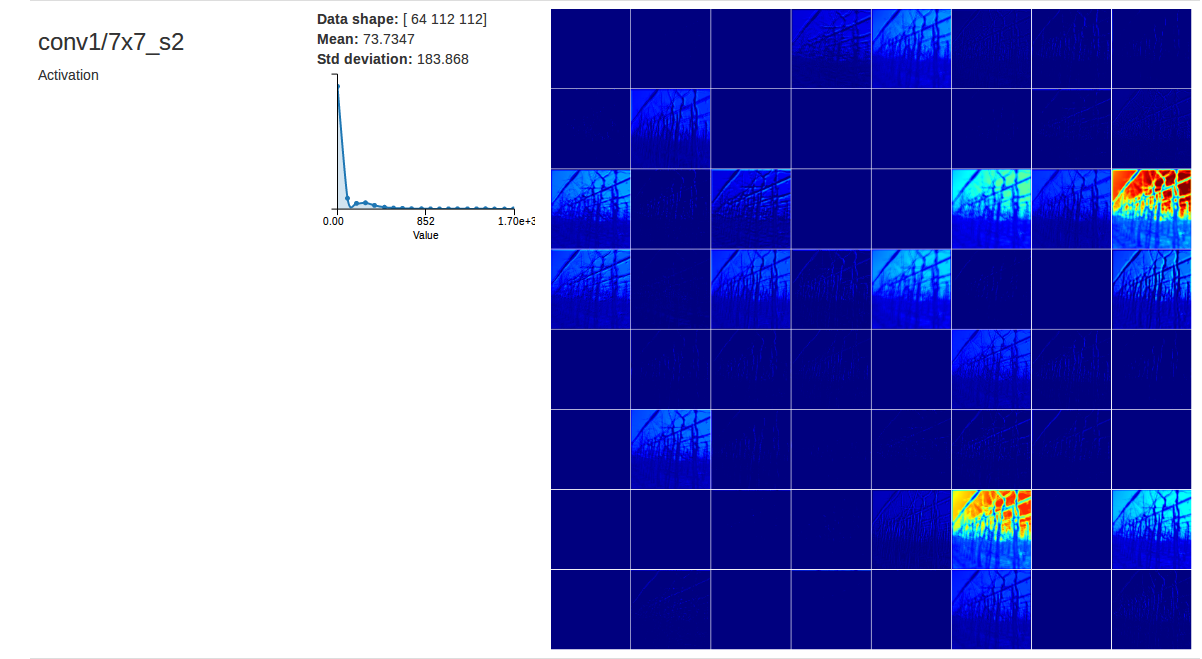
\includegraphics[width=0.45\textwidth]{right-activation}%
  }
  \caption{Activations of last convolutional layer}
\label{TS}
\end{figure}


\section{Conclusion / Future work}

\bibliography{bibliography.bib}
\bibliographystyle{ieeetr}

\end{document}
